\newpage
\section{Auswertung}
\subsection{Nullrate}
Über eine Mittelung der Messwerte der Nullrate wird jene Bestimmt als
\begin{equation}
    N_0 = 139,28 \frac{\text{Imp}}{300\text{s}}
\end{equation}
\subsection{Vanadium}
\begin{figure}
    \centering
    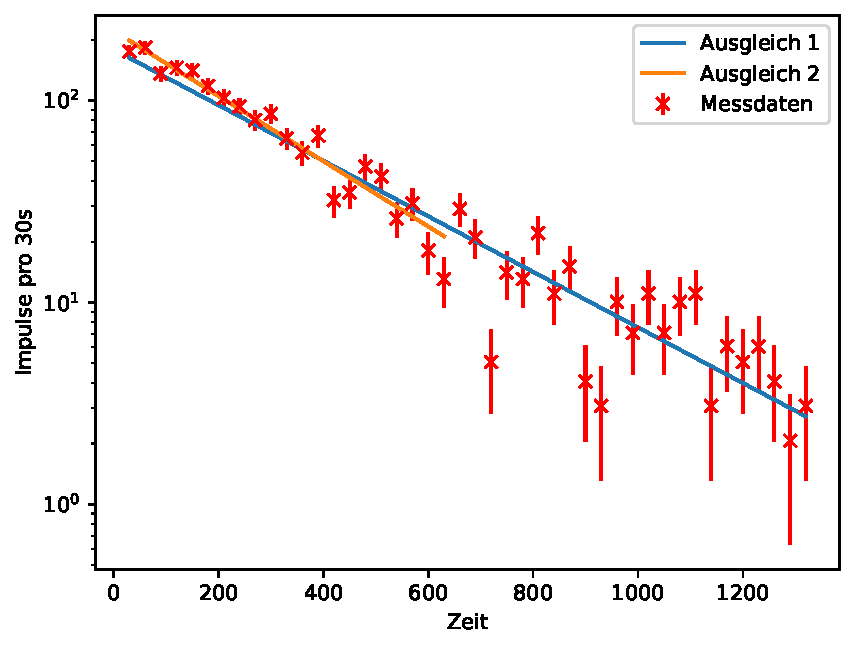
\includegraphics[width=0.7\textwidth]{plots/Vanadium.pdf}
    \caption{Ein sehr sehr toller Plot.}
\end{figure}
Mit \ref{eqn:Zerfallsgesetz} wird nun ein Ausgleich gefertigt.